\documentclass{tufte-book}%[a4paper,twoside]
% See https://github.com/Tufte-LaTeX/tufte-latex/blob/master/sample-book.tex for details

\title{Alice in Bitcoinland}
\author{Gigi}
\publisher{Do I Really Need a Publisher}

% Packages
\usepackage{lipsum}
\usepackage{booktabs}
\usepackage{graphicx}
\setkeys{Gin}{width=\linewidth,totalheight=\textheight,keepaspectratio}
\graphicspath{{graphics/}}

%%
% Just some sample text
\usepackage{lipsum}

%%
% For nicely typeset tabular material
\usepackage{booktabs}

%%
% Bibliography stuff: Biber, BibTex, BibLatex
%\usepackage[autostyle]{csquotes}
% \usepackage[
    % backend=biber,
    % style=authoryear-icomp,
    % sortlocale=de_DE,
    % natbib=true,
    % url=false,
    % doi=true,
    % eprint=false
% ]{biblatex}
% \usepackage[backend=biber]{biblatex}
\usepackage{natbib}
\bibliographystyle{abbrvnat}

%%
% Hyperlinks
\usepackage{hyperref}

%%
% For graphics / images
\usepackage{graphicx}
\setkeys{Gin}{width=\linewidth,totalheight=\textheight,keepaspectratio}
\graphicspath{{graphics/}}

% The fancyvrb package lets us customize the formatting of verbatim
% environments.  We use a slightly smaller font.
\usepackage{fancyvrb}
\fvset{fontsize=\normalsize}

%%
% Prints argument within hanging parentheses (i.e., parentheses that take
% up no horizontal space).  Useful in tabular environments.
\newcommand{\hangp}[1]{\makebox[0pt][r]{(}#1\makebox[0pt][l]{)}}

%%
% Prints an asterisk that takes up no horizontal space.
% Useful in tabular environments.
\newcommand{\hangstar}{\makebox[0pt][l]{*}}

%%
% Prints a trailing space in a smart way.
\usepackage{xspace}

% Prints the month name (e.g., January) and the year (e.g., 2008)
\newcommand{\monthyear}{%
  \ifcase\month\or January\or February\or March\or April\or May\or June\or
  July\or August\or September\or October\or November\or
  December\fi\space\number\year
}


% Prints an epigraph and speaker in sans serif, all-caps type.
\newcommand{\openepigraph}[2]{%
  %\sffamily\fontsize{14}{16}\selectfont
  \begin{fullwidth}
  \sffamily\large
  \begin{doublespace}
  \noindent\allcaps{#1}\\% epigraph
  \noindent\allcaps{#2}% author
  \end{doublespace}
  \end{fullwidth}
}

% Inserts a blank page
\newcommand{\blankpage}{\newpage\hbox{}\thispagestyle{empty}\newpage}

\usepackage{units}

% Typesets the font size, leading, and measure in the form of 10/12x26 pc.
\newcommand{\measure}[3]{#1/#2$\times$\unit[#3]{pc}}

% Macros for typesetting the documentation
\newcommand{\hlred}[1]{\textcolor{Maroon}{#1}}% prints in red
\newcommand{\hangleft}[1]{\makebox[0pt][r]{#1}}
\newcommand{\hairsp}{\hspace{1pt}}% hair space
\newcommand{\hquad}{\hskip0.5em\relax}% half quad space
\newcommand{\TODO}{\textcolor{red}{\bf TODO!}\xspace}
\newcommand{\na}{\quad--}% used in tables for N/A cells
\providecommand{\XeLaTeX}{X\lower.5ex\hbox{\kern-0.15em\reflectbox{E}}\kern-0.1em\LaTeX}
\newcommand{\tXeLaTeX}{\XeLaTeX\index{XeLaTeX@\protect\XeLaTeX}}
% \index{\texttt{\textbackslash xyz}@\hangleft{\texttt{\textbackslash}}\texttt{xyz}}
\newcommand{\tuftebs}{\symbol{'134}}% a backslash in tt type in OT1/T1
\newcommand{\doccmdnoindex}[2][]{\texttt{\tuftebs#2}}% command name -- adds backslash automatically (and doesn't add cmd to the index)
\newcommand{\doccmddef}[2][]{%
  \hlred{\texttt{\tuftebs#2}}\label{cmd:#2}%
  \ifthenelse{\isempty{#1}}%
    {% add the command to the index
      \index{#2 command@\protect\hangleft{\texttt{\tuftebs}}\texttt{#2}}% command name
    }%
    {% add the command and package to the index
      \index{#2 command@\protect\hangleft{\texttt{\tuftebs}}\texttt{#2} (\texttt{#1} package)}% command name
      \index{#1 package@\texttt{#1} package}\index{packages!#1@\texttt{#1}}% package name
    }%
}% command name -- adds backslash automatically
\newcommand{\doccmd}[2][]{%
  \texttt{\tuftebs#2}%
  \ifthenelse{\isempty{#1}}%
    {% add the command to the index
      \index{#2 command@\protect\hangleft{\texttt{\tuftebs}}\texttt{#2}}% command name
    }%
    {% add the command and package to the index
      \index{#2 command@\protect\hangleft{\texttt{\tuftebs}}\texttt{#2} (\texttt{#1} package)}% command name
      \index{#1 package@\texttt{#1} package}\index{packages!#1@\texttt{#1}}% package name
    }%
}% command name -- adds backslash automatically
\newcommand{\docopt}[1]{\ensuremath{\langle}\textrm{\textit{#1}}\ensuremath{\rangle}}% optional command argument
\newcommand{\docarg}[1]{\textrm{\textit{#1}}}% (required) command argument
\newenvironment{docspec}{\begin{quotation}\ttfamily\parskip0pt\parindent0pt\ignorespaces}{\end{quotation}}% command specification environment
\newcommand{\docenv}[1]{\texttt{#1}\index{#1 environment@\texttt{#1} environment}\index{environments!#1@\texttt{#1}}}% environment name
\newcommand{\docenvdef}[1]{\hlred{\texttt{#1}}\label{env:#1}\index{#1 environment@\texttt{#1} environment}\index{environments!#1@\texttt{#1}}}% environment name
\newcommand{\docpkg}[1]{\texttt{#1}\index{#1 package@\texttt{#1} package}\index{packages!#1@\texttt{#1}}}% package name
\newcommand{\doccls}[1]{\texttt{#1}}% document class name
\newcommand{\docclsopt}[1]{\texttt{#1}\index{#1 class option@\texttt{#1} class option}\index{class options!#1@\texttt{#1}}}% document class option name
\newcommand{\docclsoptdef}[1]{\hlred{\texttt{#1}}\label{clsopt:#1}\index{#1 class option@\texttt{#1} class option}\index{class options!#1@\texttt{#1}}}% document class option name defined
\newcommand{\docmsg}[2]{\bigskip\begin{fullwidth}\noindent\ttfamily#1\end{fullwidth}\medskip\par\noindent#2}
\newcommand{\docfilehook}[2]{\texttt{#1}\index{file hooks!#2}\index{#1@\texttt{#1}}}
\newcommand{\doccounter}[1]{\texttt{#1}\index{#1 counter@\texttt{#1} counter}}

% Generates the index
\usepackage{makeidx}
\makeindex

%%
% Chapter/Lesson Quotes
\makeatletter
\renewcommand{\@chapapp}{}% Not necessary...
\newenvironment{chapquote}[2][4em]
  {\setlength{\@tempdima}{#1}%
   \def\chapquote@author{#2}%
   \parshape 1 \@tempdima \dimexpr\textwidth-2\@tempdima\relax%
   \itshape}
  {\par\normalfont\hfill--\ \chapquote@author\hspace*{\@tempdima}\par\bigskip}
\makeatother

\begin{document}

\frontmatter

\maketitle

\cleardoublepage


%%
% Start the main matter (normal chapters)
\mainmatter

\part*{21 Lessons}

\chapter*{Introduction}
\label{ch:introduction}

\begin{chapquote}{Lewis Carroll, \textit{Alice in Wonderland}}
``But I don’t want to go among mad people,'' Alice remarked. ``Oh, you can’t
help that,'' said the Cat: ``we’re all mad here. I’m mad. You’re mad.'' ``How do
you know I’m mad?'' said Alice. ``You must be,'' said the Cat, ``or you wouldn’t
have come here.''
\end{chapquote}

In October 2018, Arjun Balaji asked the innocuous question,
\textit{What have you learned from Bitcoin?} After trying to answer this
question in a short tweet, and failing miserably, I realized that the things
I've learned are far too numerous to answer quickly, if at all.

The things I've learned are, obviously, about Bitcoin - or at least related to
it. However, while some of the inner workings of Bitcoin are explained, the
following lessons are not an explanation of how Bitcoin works or what it is,
they might, however, help to explore some of the things Bitcoin touches:
philosophical questions, economic realities, and technological innovations.

\begin{center}
  
\includegraphics[width=7cm]{assets/images/the-tweet.png}
\end{center}

The \textit{21 Lessons} are structured in bundles of seven, resulting in three
chapters. Each chapter looks at Bitcoin through a different lens, extracting
what lessons can be learned by inspecting this strange network from a different
angle.

\paragraph{\hyperref[ch:philosophy]{Chapter 1}}{explores the philosophical
teachings of Bitcoin. The interplay of immutability and change, the concept of
true scarcity, Bitcoin's immaculate conception, the problem of identity, the
contradiction of replication and locality, the power of free speech, and the
limits of knowledge.
}

\paragraph{\hyperref[ch:economics]{Chapter 2}}{explores the economic teachings
of Bitcoin. Lessons about financial ignorance, inflation, value, money and the
history of money, fractional reserve banking, and how Bitcoin is re-introducing
sound money in a sly, roundabout way.}

\paragraph{\hyperref[ch:technology]{Chapter 3}}{explores some of the lessons
learned by examining the technology of Bitcoin.  Why there is strength in
numbers, reflections on trust, why telling time takes work, how moving slowly
and not breaking things is a feature and not a bug, what Bitcoin's creation can
tell us about privacy, why cypherpunks write code (and not laws), and what
metaphors might be useful to explore Bitcoin's future.}

~

Each lesson contains several quotes and links throughout the text. If an idea is
worth exploring in more detail, you can follow the links to related works in the
footnotes or in the bibliography.

Even though some prior knowledge about Bitcoin is beneficial, I hope that these
lessons can be digested by any curious reader. While some relate to each other,
each lesson should be able to stand on its own and can be read independently. I
did my best to shy away from technical jargon, even though some domain-specific
vocabulary is unavoidable.

I hope that my writing serves as inspiration for others to dig beneath the
surface and examine some of the deeper questions Bitcoin raises. My own
inspiration came from a multitude of authors and content creators to all of whom
I am eternally grateful.

Last but not least: my goal in writing this is not to convince you of anything.
My goal is to make you think, and show you that there is way more to Bitcoin
than meets the eye. I can’t even tell you what Bitcoin is or what Bitcoin will
teach you. You will have to find that out for yourself.

\begin{samepage}\begin{quotation}
\enquote{After this, there is no turning back. You take the blue pill --- the
story ends, you wake up in your bed and believe whatever you want to
believe. You take the red pill\footnote{the \textit{orange} pill} --- you stay in Wonderland, and I show
you how deep the rabbit hole goes.}
\flushright -- Morpheus
\end{quotation}\end{samepage}

\begin{figure}
  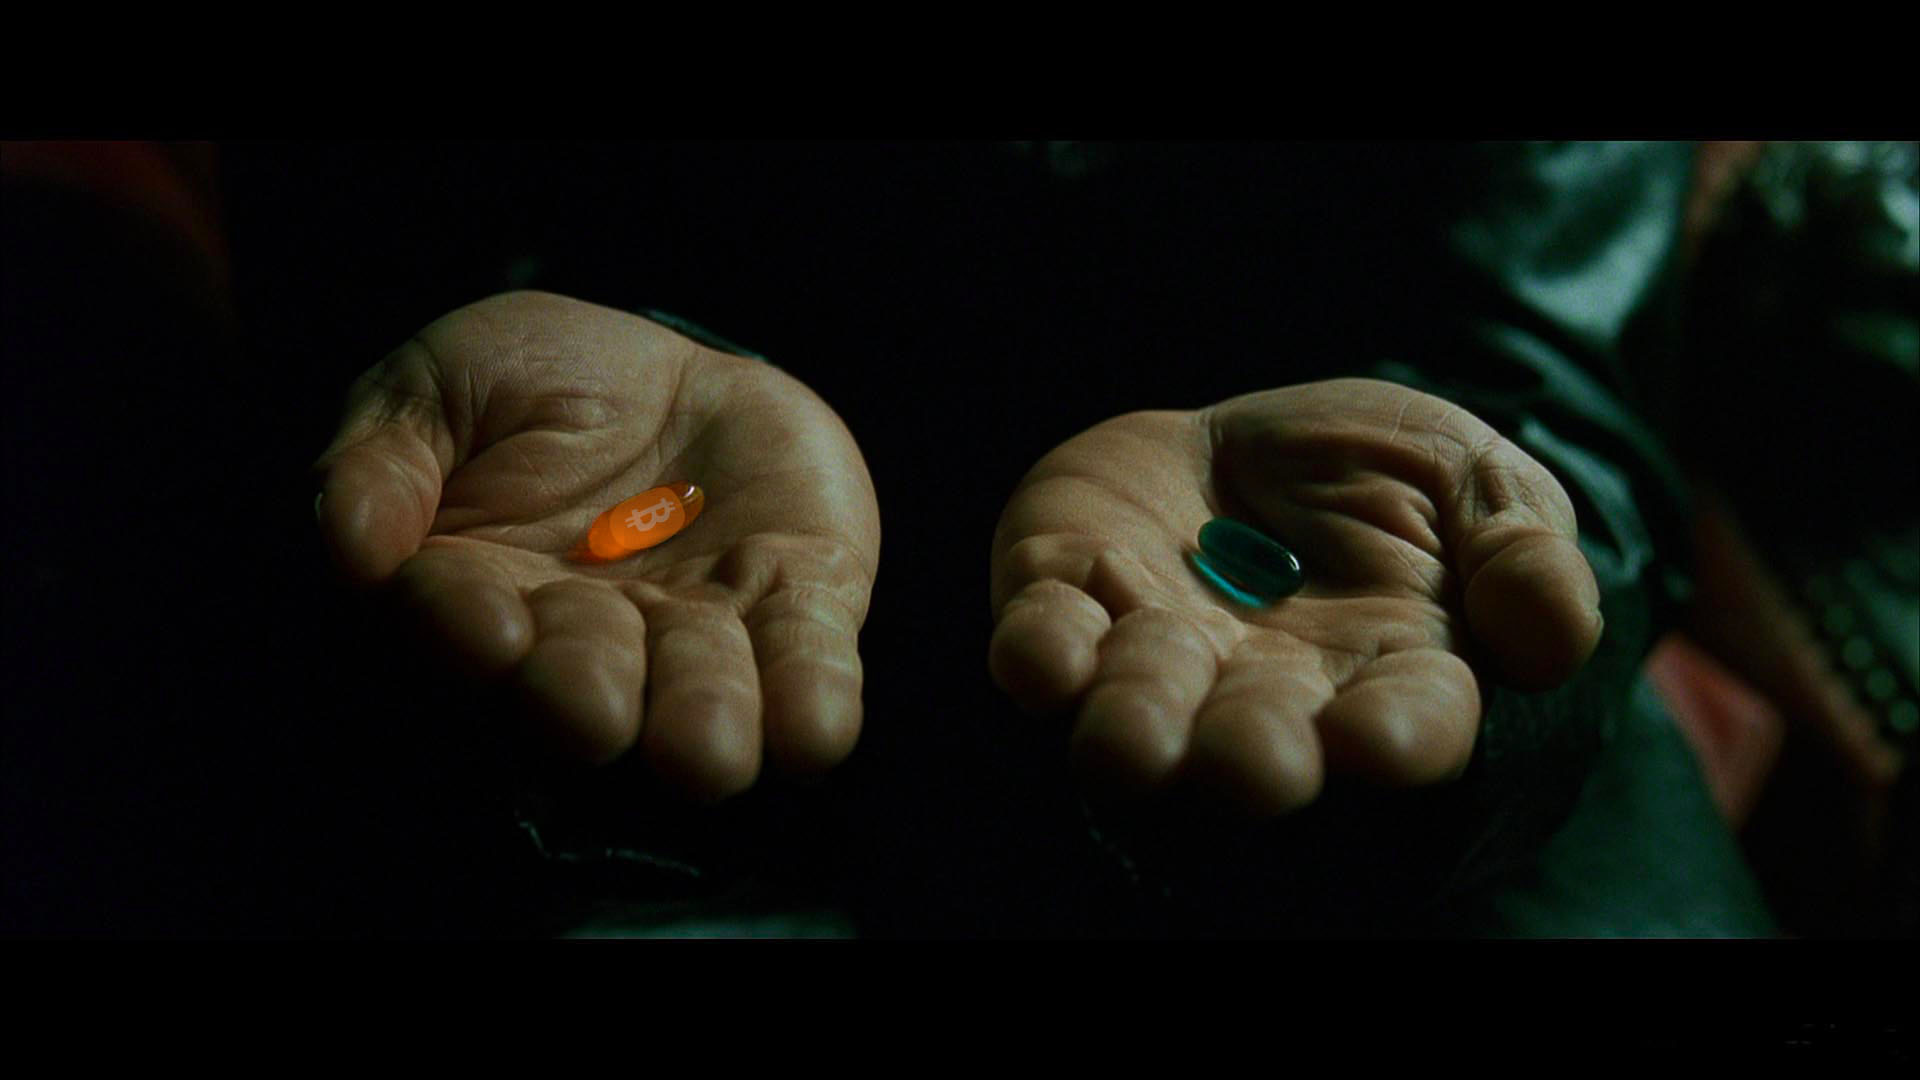
\includegraphics{assets/images/bitcoin-orange-pill.jpg}
  \caption*{Remember: All I'm offering is the truth. Nothing more.}
  \label{fig:bitcoin-orange-pill}
\end{figure}

%
% [Morpheus]: https://en.wikipedia.org/wiki/Red_pill_and_blue_pill#The_Matrix_(1999)
% [this question]: https://twitter.com/arjunblj/status/1050073234719293440
%
% <!-- Internal -->
% [chapter1]: {{ 'bitcoin/lessons/ch1-00-philosophy' | absolute_url }}
% [chapter2]: {{ 'bitcoin/lessons/ch2-00-economics' | absolute_url }}
% [chapter3]: {{ 'bitcoin/lessons/ch3-00-technology' | absolute_url }}
%
% <!-- Wikipedia -->
% [alice]: https://en.wikipedia.org/wiki/Alice%27s_Adventures_in_Wonderland
% [carroll]: https://en.wikipedia.org/wiki/Lewis_Carroll

\part{Philosophy}
\label{ch:philosophy}

% \blockquote{
% The mouse looked at her rather inquisitively, and seemed to her to wink with one
% of its little eyes, but it said nothing.
% }
%
% \newthought{Looking at Bitcoin} superficially, one might conclude that it is slow, wasteful,
% unnecessarily redundant, and overly paranoid. Looking at Bitcoin inquisitively,
% one might find out that things are not as they seem at first glance.

Bitcoin has a way of taking your assumptions and turning them on their heads.
After a while, just when you were about to get comfortable again, Bitcoin will
smash through the wall like a bull in a china shop and shatter your assumptions
once more.

\begin{figure}
  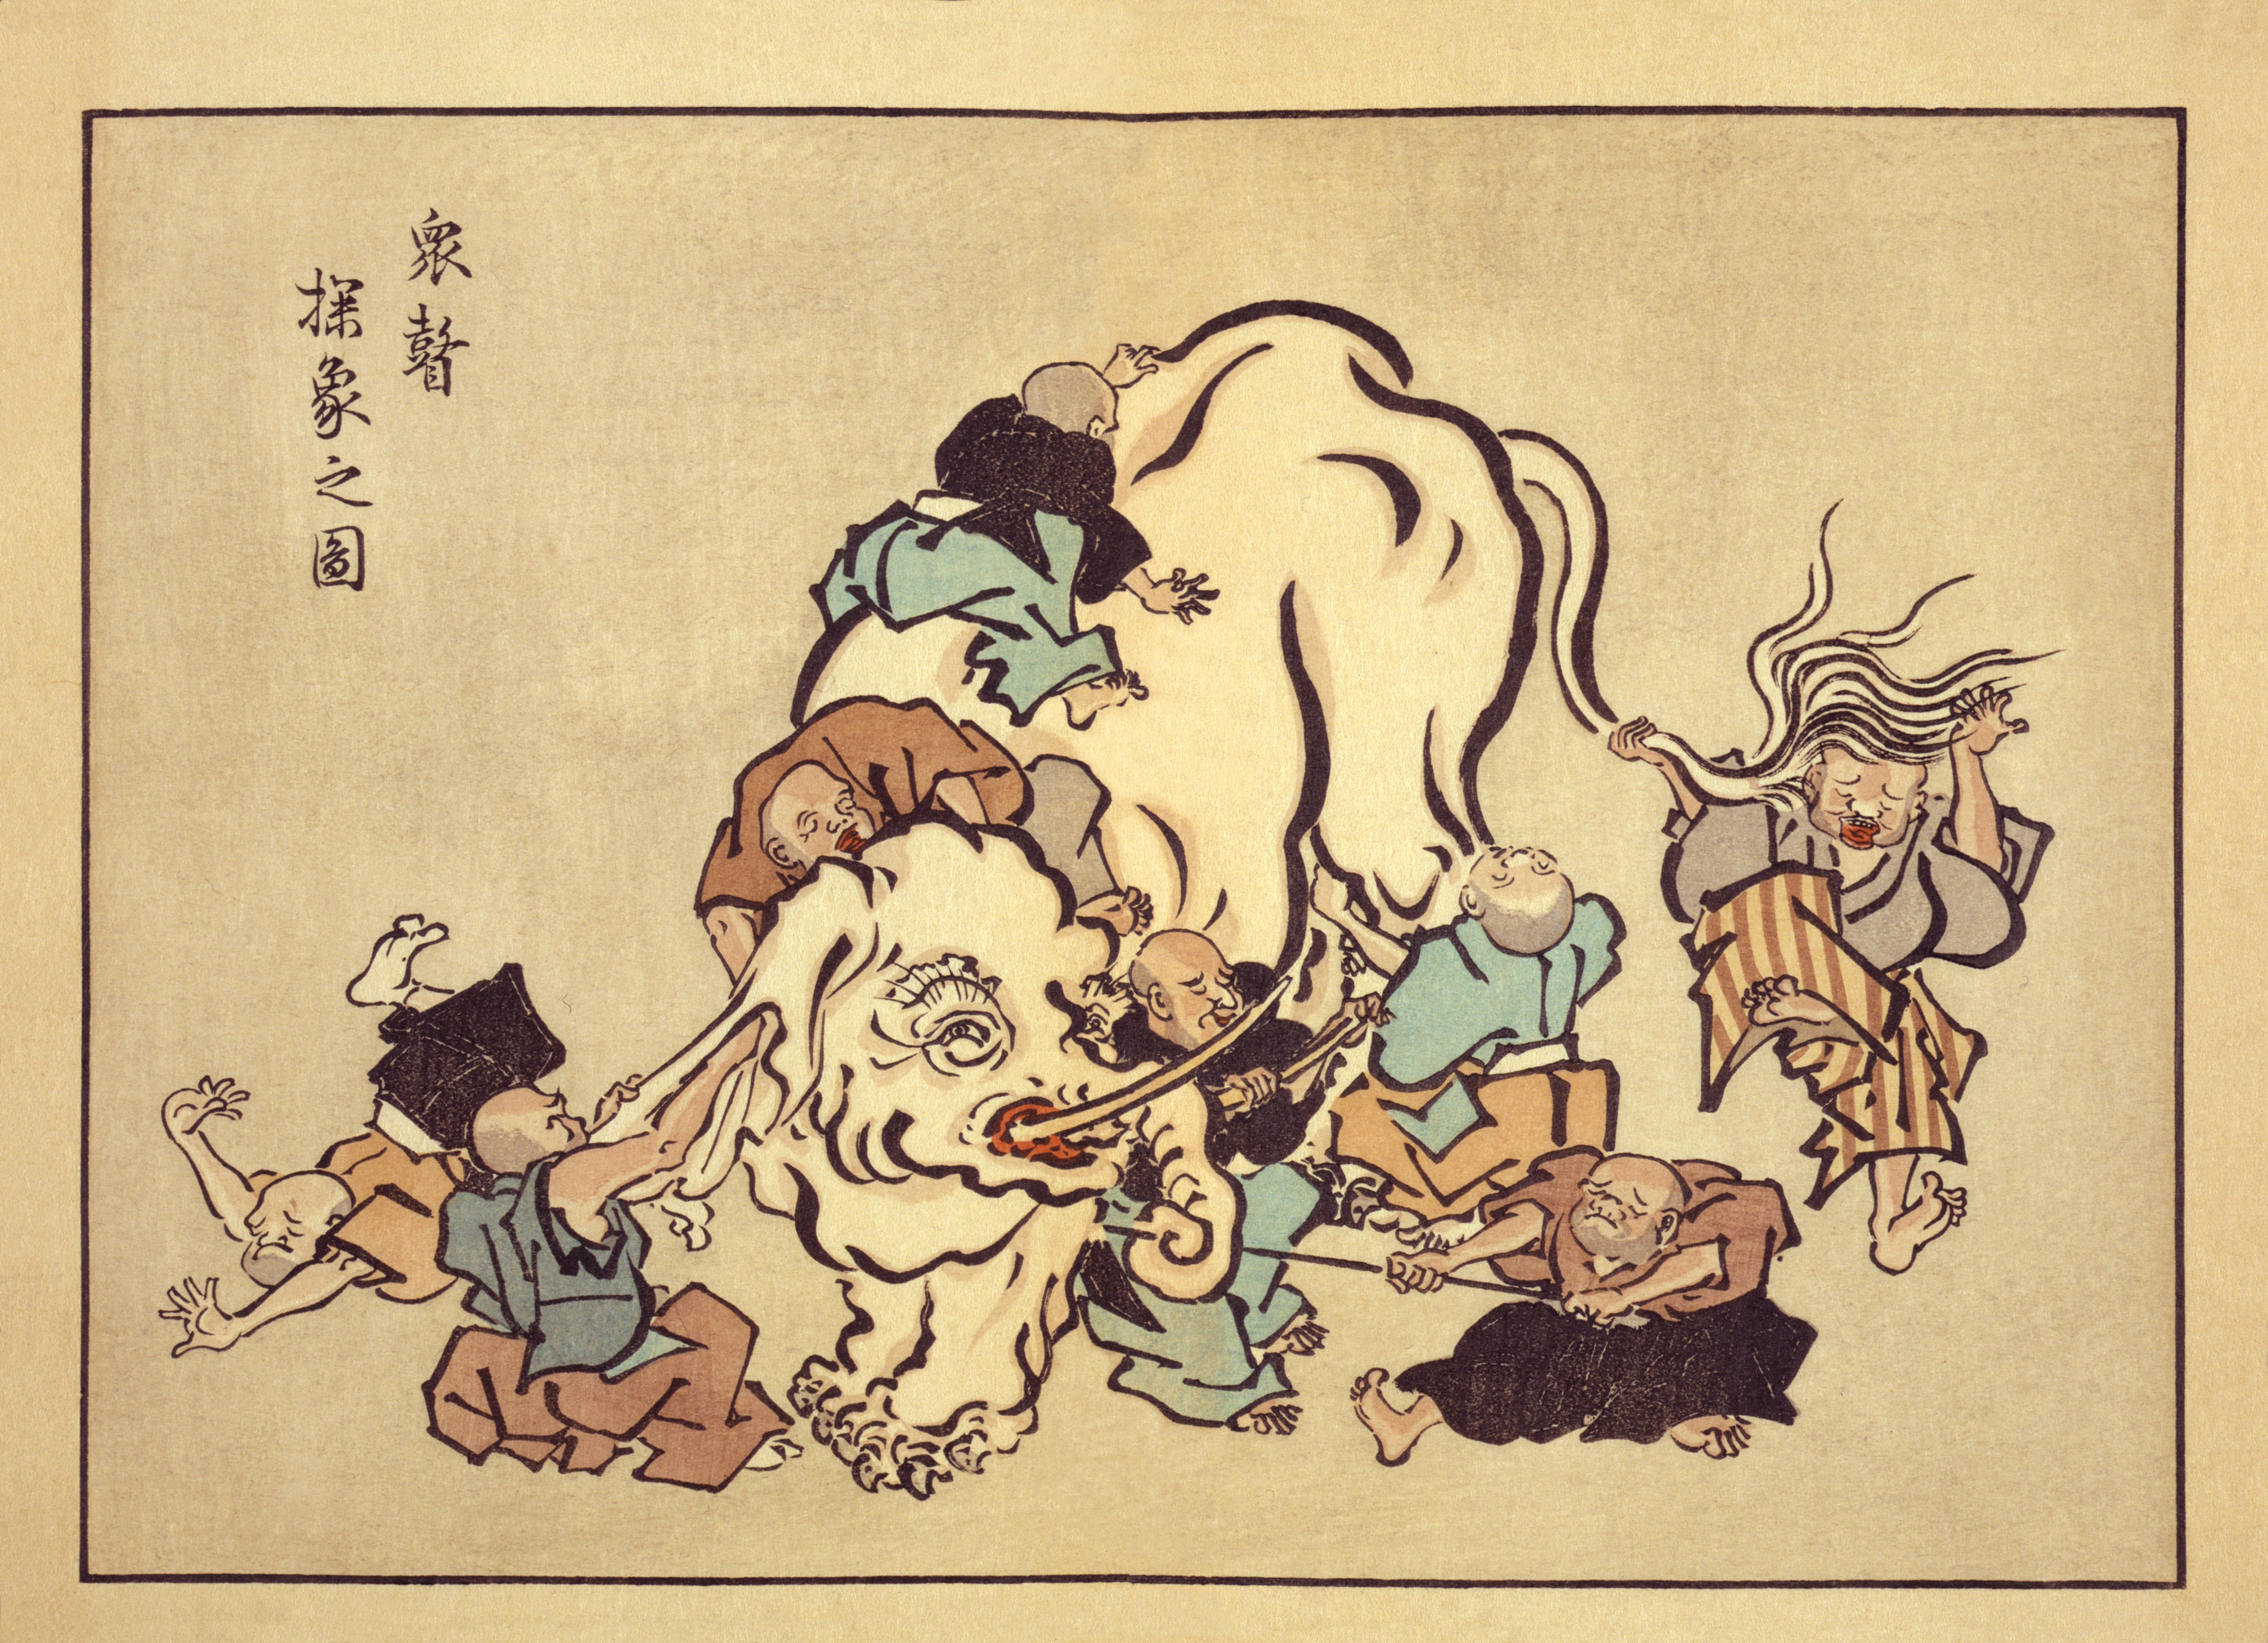
\includegraphics{assets/images/blind-monks.jpg}
  \caption{Blind monks examining the Bitcoin bull}
  \label{fig:blind-monks}
\end{figure}

Bitcoin is a child of many disciplines. Like blind monks examining an elephant,
everyone who approaches this novel technology does so from a different angle.
And everyone will come to different conclusions about the nature of the beast.

The following lessons are about some of my assumptions which Bitcoin shattered,
and the conclusions I arrived at. Philosophical questions of immutability,
scarcity, locality, and identity are explored in the first four lessons.

TODO: Lesson List
% 

Lesson 5 explores how Bitcoin's origin story is not only fascinating but
absolutely essential for a leaderless system. The last two lessons of this
chapter explore the power of free speech and the limits of our individual
knowledge, reflected by the surprising depth of the Bitcoin rabbit hole.

I hope that you will find the world of Bitcoin as educational, fascinating and
entertaining as I did and still do. I invite you to follow the white rabbit and
explore the depths of this rabbit hole. Now hold on to your pocket watch, pop
down, and enjoy the fall.

\chapter{Immutability and Change}
\label{les:1}

\begin{chapquote}{Alice}
\enquote{I wonder if I've been changed in the night. Let me think. Was I the same when I
got up this morning? I almost think I can remember feeling a little different.
But if I'm not the same, the next question is `Who in the world am I?' Ah,
that's the great puzzle!}
\end{chapquote}

Bitcoin is inherently hard to describe. It is a \textit{new thing}, and any
attempt to draw a comparison to previous concepts -- be it by calling
it digital gold or the internet of money -- is bound to fall short of
the whole. Whatever your favorite analogy might be, two aspects of
Bitcoin are absolutely essential: decentralization and immutability.

\paragraph{}
One way to think about Bitcoin is as an automated social contract\footnote{Hasu,
Unpacking Bitcoin's Social Contract~\cite{social-contract}}. The software is
just one piece of the puzzle, and hoping to change Bitcoin by changing the
software is an exercise in futility. One would have to convince the rest of the
network to adopt the changes, which is more a psychological effort than a
software engineering one.

\paragraph{}
The following might sound absurd at first, like so many other things in
this space, but I believe that it is profoundly true nonetheless: You
won't change Bitcoin, but Bitcoin will change you.

\begin{quotation}\begin{samepage}
\enquote{Bitcoin will change us more than we will change it.}
\begin{flushright} -- Marty Bent\footnote{Tales From the Crypt~\cite{tftc21}}
\end{flushright}\end{samepage}\end{quotation}

It took me a long time to realize the profundity of this. Since Bitcoin
is just software and all of it is open-source, you can simply change
things at will, right? Wrong. \textit{Very} wrong. Unsurprisingly, Bitcoin's
creator knew this all too well.

\begin{quotation}\begin{samepage}
\enquote{The nature of Bitcoin is such that once version 0.1 was released, the core
design was set in stone for the rest of its lifetime.}
\begin{flushright} -- Satoshi Nakamoto\footnote{BitcoinTalk forum post: `Re:
Transactions and Scripts\ldots'~\cite{satoshi-set-in-stone}}
\end{flushright}\end{samepage}\end{quotation}

Many people have attempted to change Bitcoin's nature. So far all of
them have failed. While there is an endless sea of forks and altcoins,
the Bitcoin network still does its thing, just as it did when the first
node went online. The altcoins won't matter in the long run. The forks
will eventually starve to death. Bitcoin is what matters. As long as our
fundamental understanding of mathematics and/or physics doesn't change,
the Bitcoin honeybadger will continue to not care.

\begin{quotation}\begin{samepage}
\enquote{Bitcoin is the first example of a new form of life. It lives and
breathes on the internet. It lives because it can pay people to keep
it alive. [\ldots] It can't be changed. It can't be argued with. It
can't be tampered with. It can't be corrupted. It can't be stopped.
[\ldots] If nuclear war destroyed half of our planet, it would continue
to live, uncorrupted.}
\begin{flushright} -- Ralph Merkle\footnote{DAOs, Democracy and
Governance,~\cite{merkle-dao}}
\end{flushright}\end{samepage}\end{quotation}

The heartbeat of the Bitcoin network will outlast all of ours.

~

Realizing the above changed me way more than the past blocks of the Bitcoin
blockchain ever will. It changed my time preference, my understanding of
economics, my political views, and so much more. Hell, it is even changing
people's diets\footnote{Inside the World of the Bitcoin
Carnivores,~\cite{carnivores}}. If all of this sounds crazy to you, you're in
good company. All of this is crazy, and yet it is happening.

~

\paragraph{Bitcoin taught me that it won't change. I will.}

% ---
%
% #### Through the Looking-Glass
%
% - [Bitcoin's Gravity: How idea-value feedback loops are pulling people in][gravity]
% - [Lesson 18: Move slowly and don't break things][lesson18]
%
% #### Down the Rabbit Hole
%
% - [Unpacking Bitcoin's Social Contract][automated social contract]: A framework for skeptics by Hasu
% - [DAOs, Democracy and Governance][Ralph Merkle] by Ralph C. Merkle
% - [Marty's Bent][bent]: A daily newsletter highlighting signal in Bitcoin by Marty Bent
% - [Technical Discussion on Bitcoin's Transactions and Scripts][Satoshi Nakamoto] by Satoshi Nakamoto, Gavin Andresen, and others
% - [Inside the World of the Bitcoin Carnivores][carnivores]: Why a small community of Bitcoin users is eating meat exclusively by Jordan Pearson
% - [Tales From the Crypt][tftc] hosted by Marty Bent
%
% <!-- Internal -->
% [gravity]: 
% [lesson18]: {{ 'bitcoin/lessons/ch3-18-move-slowly-and-dont-break-things' | absolute_url }}
%
% <!-- Further Reading -->
% [automated social contract]: https://medium.com/@hasufly/bitcoins-social-contract-1f8b05ee24a9
% [carnivores]: https://motherboard.vice.com/en_us/article/ne74nw/inside-the-world-of-the-bitcoin-carnivores
% [tftc]: https://tftc.io/tales-from-the-crypt/
% [bent]: https://tftc.io/martys-bent/
%
% <!-- Quotes -->
% [Ralph Merkle]: http://merkle.com/papers/DAOdemocracyDraft.pdf
% [Satoshi Nakamoto]: https://bitcointalk.org/index.php?topic=195.msg1611#msg1611
%
% <!-- Twitter People -->
% [Marty Bent]: https://twitter.com/martybent
%
% <!-- Wikipedia -->
% [alice]: https://en.wikipedia.org/wiki/Alice%27s_Adventures_in_Wonderland
% [carroll]: https://en.wikipedia.org/wiki/Lewis_Carroll


\chapter{ The Scarcity of Scarcity}
\label{les:2}

\begin{chapquote}{Alice}
That's quite enough - I hope I sha'n't grow any more...
\end{chapquote}

In general, the advance of technology seems to make things more abundant. More
and more people are able to enjoy what previously have been luxurious goods.
Soon, we will all live like kings. Most of us already do. As Peter Diamandis
wrote in Abundance\cite{abundance}: ``Technology is a resource-liberating
mechanism. It can make the once scarce the now abundant.''

Bitcoin, an advanced technology in itself, breaks this trend and creates
a new commodity which is truly scarce. Some even argue that it is one of
the scarcest things in the universe. The supply can't be inflated, no
matter how much effort one chooses to expend towards creating more.

\begin{chapquote}{\cite{bitcoinstandard-pres}}
``Only two things are genuinely scarce: time and
bitcoin.''
\end{chapquote}

Paradoxically, it does so by a mechanism of copying. Transactions are
broadcast, blocks are propagated, the distributed ledger is --- well,
you guessed it --- distributed. All of these are just fancy words for
copying. Heck, Bitcoin even copies itself onto as many computers as it
can, by incentivizing individual people to run full nodes and mine new
blocks.

All of this duplication wonderfully works together in a concerted effort
to produce scarcity.

In a time of abundance, Bitcoin taught me what real scarcity is.

% ---
%
% #### Through the Looking-Glass
%
% - [Lesson 14: Sound money][lesson14]
%
% #### Down the Rabbit Hole
%
% - [The Bitcoin Standard: The Decentralized Alternative to Central Banking][bitcoin-standard]
% - [Abundance: The Future Is Better Than You Think][Abundance] by Peter Diamandis
% - [Presentation on The Bitcoin Standard][bitcoin-standard-presentation] by Saifedean Ammous
% - [Modeling Bitcoin's Value with Scarcity][planb-scarcity] by PlanB
% - 🎧 [Misir Mahmudov on the Scarcity of Time & Bitcoin][tftc60] TFTC #60 hosted by Marty Bent
% - 🎧 [PlanB – Modelling Bitcoin's digital scarcity through stock-to-flow techniques][slp67] SLP #67 hosted by Stephan Livera
%
% <!-- Through the Looking-Glass -->
% [lesson14]: {{ 'bitcoin/lessons/ch2-14-sound-money' | absolute_url }}
%
% <!-- Down the Rabbit Hole -->
% [Abundance]: https://www.diamandis.com/abundance
% [bitcoin-standard]: http://amzn.to/2L95bJW
% [bitcoin-standard-presentation]: https://www.bayernlb.de/internet/media/de/ir/downloads_1/bayernlb_research/sonderpublikationen_1/bitcoin_munich_may_28.pdf
% [planb-scarcity]: https://medium.com/@100trillionUSD/modeling-bitcoins-value-with-scarcity-91fa0fc03e25
% [tftc60]: https://anchor.fm/tales-from-the-crypt/episodes/Tales-from-the-Crypt-60-Misir-Mahmudov-e3aibh
% [slp67]: https://stephanlivera.com/episode/67
%
% <!-- Wikipedia -->
% [alice]: https://en.wikipedia.org/wiki/Alice%27s_Adventures_in_Wonderland
% [carroll]: https://en.wikipedia.org/wiki/Lewis_Carroll

\chapter{Replicação e Localidade}
\label{les:3}

\begin{chapquote}{Lewis Carroll, \textit{Alice no País das Maravilhas}}
Em seguida uma voz irada, do Coelho: \enquote{Pat, Pat! onde você está?}
\end{chapquote}

Deixando a mecânica quântica de lado, a localidade não é um problema no mundo físico. A questão \textit{\enquote{Onde está X?}} Pode ser respondida de forma significativa, não importa se X é uma pessoa ou um objeto. No mundo digital, a pergunta do \textit{onde} já é mais complicada, mas não impossível de responder. Onde estão seus e-mails realmente? Uma resposta não muito boa seria \enquote{na nuvem} que nada mais é que o computador de outra pessoa. Ainda assim, se você quisesse rastrear cada dispositivo de armazenamento que contém seus e-mails, você poderia, em teoria, localizá-los.

Com o bitcoin, a pergunta do \enquote{onde} é \textit{realmente} complicada. Onde, exatamente, estão seus bitcoins?

\begin{quotation}\begin{samepage}
\enquote{Abri os olhos, olhei em volta e fiz a pergunta inevitável, tradicional e lamentavelmente banal do pós-operatório: "Onde estou?"}
\begin{flushright} -- Daniel Dennett\footnote{Daniel Dennett, \textit{Where Am I?}~\cite{where-am-i}}
\end{flushright}\end{samepage}\end{quotation}

O problema é duplo. Primeiro, o livro-razão distribuído é distribuído por replicação completa, o que significa que ele está em toda parte. Em segundo lugar, não existem bitcoins. Não apenas fisicamente, mas \textit{tecnicamente}.

O Bitcoin rastreia um conjunto de saídas de transações não gastas, sem nunca ter que se referir a uma entidade que represente um bitcoin. A existência de um bitcoin é baseada observando-se o conjunto de saídas de transações não gastas e chamando cada entrada com 100 milhões de unidades básicas de bitcoin.

\begin{quotation}\begin{samepage}
\enquote{Onde está, neste momento, em trânsito? [...] primeiro, não há bitcoins. Simplesmente não existem. Eles não existem. Existem entradas em um livro-razão que é compartilhado [...] Eles não existem em nenhum local físico. O livro-razão existe em todos os locais físicos, essencialmente. A geografia não faz sentido neste mundo --- não vai ajudá-lo a descobrir a sua política aqui.}
\begin{flushright} -- Peter Van Valkenburgh\footnote{Peter Van Valkenburgh on the \textit{What Bitcoin Did} podcast, episode 49 \cite{wbd049}}
\end{flushright}\end{samepage}\end{quotation}

Então, o que você realmente possui quando diz \textit{\enquote{Eu tenho um bitcoin}} se não há bitcoins? Bem, lembra de todas essas palavras estranhas que você foi forçado a escrever quando usou uma carteira? Acontece que essas palavras mágicas são o que você realmente possui: um feitiço mágico \footnote{The Magic Dust of Cryptography: Como a informação digital está mudando nossa sociedade \cite{gigi:magic-spell}} que pode ser usado para adicionar algumas entradas ao livro-razão público --- as chaves para \enquote{mover} alguns bitcoins. É por isso que, para todos os efeitos, suas chaves privadas \textit{são} seus bitcoins. Se você acha que estou inventando tudo isso, sinta-se à vontade para me enviar suas chaves privadas.

\paragraph{O Bitcoin me ensinou que localidade é um negócio complicado.}

% ---
%
% #### Through the Looking-Glass
%
% - [The Magic Dust of Cryptography: How digital information is changing our society][a magic spell]
%
% #### Down the Rabbit Hole
%
% - [Where Am I?][Daniel Dennett] by Daniel Dennett
% - 🎧 [Peter Van Valkenburg on Preserving the Freedom to Innovate with Public Blockchains][wbd049] WBD #49 hosted by Peter McCormack
%
% <!-- Through the Looking-Glass -->
% [a magic spell]: 
%
% <!-- Down the Rabbit Hole -->
% [Daniel Dennett]: https://www.lehigh.edu/~mhb0/Dennett-WhereAmI.pdf
% [1st Amendment]: https://en.wikipedia.org/wiki/First_Amendment_to_the_United_States_Constitution
% [wbd049]: https://www.whatbitcoindid.com/podcast/coin-centers-peter-van-valkenburg-on-preserving-the-freedom-to-innovate-with-public-blockchains
%
% <!-- Wikipedia -->
% [alice]: https://en.wikipedia.org/wiki/Alice%27s_Adventures_in_Wonderland
% [carroll]: https://en.wikipedia.org/wiki/Lewis_Carroll

\chapter{The Problem of Identity}
\label{les:4}

\begin{chapquote}{Lewis Carroll, \textit{Alice in Wonderland}}
  \enquote{Who are you?} said the caterpillar.
\end{chapquote}

Nic Carter, in an homage to Thomas Nagel's treatment of the same
question in regards to a bat, wrote an excellent piece which discusses
the following question: What is it like to be a bitcoin? He
brilliantly shows that open, public blockchains in general, and Bitcoin
in particular, suffer from the same conundrum as the Ship of
Theseus: which Bitcoin is the real Bitcoin?

\begin{quotation}\begin{samepage}
\enquote{Consider just how little persistence Bitcoin's components have. The
entire codebase has been reworked, altered, and expanded such that it
barely resembles its original version. [...] The registry of who
owns what, the ledger itself, is virtually the only persistent trait
of the network [...]
To be considered truly leaderless, you must surrender the easy
solution of having an entity that can designate one chain as the
legitimate one.}
\begin{flushright} -- Nic Carter\footnote{Nic Carter, \textit{What is it like to be a bitcoin?} \cite{bitcoin-identity}}
\end{flushright}\end{samepage}\end{quotation}

It seems like the advancement of technology keeps forcing us to take
these philosophical questions seriously. Sooner or later, self-driving
cars will be faced with real-world versions of the trolley problem,
forcing them to make ethical decisions about whose lives do matter and
whose do not.

Cryptocurrencies, especially since the first contentious hard-fork,
force us to think about and agree upon the metaphysics of identity.
Interestingly, the two biggest examples we have so far have lead to two
different answers. On August 1, 2017, Bitcoin split into two camps. The
market decided that the unaltered chain is the original Bitcoin. One
year earlier, on October 25, 2016, Ethereum split into two camps. The
market decided that the \textit{altered} chain is the original Ethereum.

If properly decentralized, the questions posed by the \textit{Ship of Theseus}
will have to be answered in perpetuity for as long as these networks of
value-transfer exist.

\paragraph{Bitcoin taught me that decentralization contradicts identity.}

% ---
%
% #### Down the Rabbit Hole
%
% - [What Is It Like to be a Bat?][in regards to a bat] by Thomas Nagel
% - [What is it like to be a bitcoin?] by Nic Carter
% - [Ship of Theseus], [trolley problem] on Wikipedia
%
% [in regards to a bat]: https://en.wikipedia.org/wiki/What_Is_it_Like_to_Be_a_Bat%3F
% [What is it like to be a bitcoin?]: https://medium.com/s/story/what-is-it-like-to-be-a-bitcoin-56109f3e6753
% [Ship of Theseus]: https://en.wikipedia.org/wiki/Ship_of_Theseus
% [trolley problem]: https://en.wikipedia.org/wiki/Trolley_problem
%
% <!-- Wikipedia -->
% [alice]: https://en.wikipedia.org/wiki/Alice%27s_Adventures_in_Wonderland
% [carroll]: https://en.wikipedia.org/wiki/Lewis_Carroll

\chapter{Uma concepção imaculada}
\label{les:5}

\begin{chapquote}{Lewis Carroll, \textit{Alice no País das Maravilhas}}
\enquote{Suas cabeças se foram, para servi-la, Majestade}, os soldados gritaram em resposta\ldots
\end{chapquote}

Todo mundo adora uma boa história de origem. A história de origem do Bitcoin é fascinante, e os detalhes dela são mais importantes do que se possa pensar quando sabemos pela primeira vez. Quem é Satoshi Nakamoto? Ele era uma pessoa ou um grupo de pessoas? Ele era ela? Seria um alien viajando no tempo ou IA avançada? Deixando de lado as teorias estranhas, provavelmente nunca saberemos. E isso é importante.

O Satoshi escolheu ser anônimo. Ele plantou a semente do Bitcoin. Ele ficou por aqui por tempo suficiente para garantir que a rede não morresse quando estava engatinhando. E então ele desapareceu.

O que pode parecer um golpe estranho de anonimato é realmente crucial para um sistema verdadeiramente descentralizado. Sem controle centralizado. Nenhuma autoridade centralizada. Nenhum inventor. Ninguém para processar, torturar, chantagear ou extorquir. Uma concepção imaculada de tecnologia.

\begin{quotation}\begin{samepage}
\enquote{Uma das melhores coisas que Satoshi fez foi desaparecer.}
\begin{flushright} -- Jimmy Song\footnote{Jimmy Song, \textit{Por que o Bitcoin é Diferente} \cite{bitcoin-different}}
\end{flushright}\end{samepage}\end{quotation}

\newpage

Desde o nascimento do Bitcoin, milhares de outras criptomoedas foram criadas. Nenhum desses clones compartilha sua história de origem. Se você quiser substituir o Bitcoin, terá que transcender sua história de origem. Em uma guerra de ideias, as narrativas ditam a sobrevivência.

\begin{quotation}\begin{samepage}
\enquote{O ouro foi transformado pela primeira vez em joias e usado para troca há mais de 7.000 anos. O brilho cativante do ouro o levou a ser considerado um presente
dos deuses.}
\begin{flushright} Austrian Mint\footnote{The Austrian Mint, \textit{Gold: The Extraordinary Metal} \cite{gold-gift-gods}}
\end{flushright}\end{samepage}\end{quotation}

Como o ouro nos tempos antigos, o Bitcoin pode ser considerado um presente dos deuses. Ao contrário do ouro, as origens dos Bitcoins são muito humanas. E desta vez, sabemos quem são os deuses do desenvolvimento e da manutenção: pessoas de todo o mundo, anônimas ou não.

\paragraph{O Bitcoin me ensinou que narrativas são importantes.}

% ---
%
% #### Down the Rabbit Hole
%
% - [Why Bitcoin is different][Jimmy Song] by Jimmy Song
% - [Gold: The Extraordinary Metal] by the Austrian Mint
%
% <!-- Down the Rabbit Hole -->
% [Jimmy Song]: https://medium.com/@jimmysong/why-bitcoin-is-different-e17b813fd947
% [Gold: The Extraordinary Metal]: https://www.muenzeoesterreich.at/eng/discover/for-investors/gold-the-extraordinary-metal
%
% <!-- Wikipedia -->
% [alice]: https://en.wikipedia.org/wiki/Alice%27s_Adventures_in_Wonderland
% [carroll]: https://en.wikipedia.org/wiki/Lewis_Carroll

\chapter{The Power of Free Speech}
\label{les:6}

\begin{chapquote}{Lewis Carroll, \textit{Alice in Wonderland}}
``I beg your pardon?'' said the mouse, frowning, but very politely, ``did you speak?''
\end{chapquote}

Bitcoin is an idea. An idea which, in its current form, is the
manifestation of a machinery purely powered by text. Every aspect of
Bitcoin is text: The whitepaper is text. The software which is run by
its nodes is text. The ledger is text. Transactions are text. Public and
private keys are text. Every aspect of Bitcoin is text, and thus
equivalent to speech.

\begin{quotation}
``Congress shall make no law respecting an establishment of religion,
or prohibiting the free exercise thereof; or abridging the freedom of
speech, or of the press; or the right of the people peaceably to
assemble, and to petition the Government for a redress of grievances.''
\flushright -- First Amendment to the U.S. Constitution
\end{quotation}
% > <cite>[First Amendment to the United States Constitution][1st Amendment]</cite>

Although the final battle of the [Crypto Wars] has not been fought yet,
it will be very difficult to criminalize an idea, let alone an idea
which is based on the exchange of text messages. Every time a government
tries to outlaw text or speech, we slip down a path of absurdity which
inevitably leads to abominations like [illegal numbers] and [illegal
primes].

As long as there is a part of the world where speech is free as in
\textit{freedom}, Bitcoin is unstoppable.

\begin{quotation}
``There is no point in any Bitcoin transaction that Bitcoin ceases to be
\textbf{text}. It is \textbf{all text}, all the time. [...] Bitcoin is
\textbf{text}. Bitcoin is \textbf{speech}. It cannot be regulated in a free
country like the USA with guaranteed inalienable rights and a First Amendment
that explicitly excludes the act of publishing from government oversight.''
\end{quotation}
% > <cite>[Beautyon]</cite>

\paragraph{Bitcoin taught me that in a free society, free speech and free software
are unstoppable.}

% ---
%
% #### Through the Looking-Glass
%
% - [The Magic Dust of Cryptography: How digital information is changing our society][a magic spell]
%
% #### Down the Rabbit Hole
%
% - [Why America can't regulate Bitcoin][Beautyon] by Beautyon
% - [First Amendment to the United States Constitution][1st Amendment], [Crypto Wars], [illegal numbers], [illegal primes] on Wikipedia
%
% <!-- Through the Looking-Glass -->
% [a magic spell]: 
%
% <!-- Down the Rabbit Hole -->
% [1st Amendment]: https://en.wikipedia.org/wiki/First_Amendment_to_the_United_States_Constitution
% [Crypto Wars]: https://en.wikipedia.org/wiki/Crypto_Wars
% [illegal numbers]: https://en.wikipedia.org/wiki/Illegal_number
% [illegal primes]: https://en.wikipedia.org/wiki/Illegal_prime
% [Beautyon]: https://hackernoon.com/why-america-cant-regulate-bitcoin-8c77cee8d794
%
% <!-- Wikipedia -->
% [alice]: https://en.wikipedia.org/wiki/Alice%27s_Adventures_in_Wonderland
% [carroll]: https://en.wikipedia.org/wiki/Lewis_Carroll

\chapter{ The Limits of Knowledge}
\label{les:7}

\begin{chapquote}{Lewis Carroll, \textit{Alice in Wonderland}}
``Down, down, down. Would the fall never come to an end?''
\end{chapquote}

Getting into Bitcoin is a humbling experience. I thought that I knew
things. I thought that I was educated. I thought that I knew my computer
science, at the very least. I studied it for years, so I have to know
everything about digital signatures, hashes, encryption, operational
security, and networks, right?

Wrong.

Learning all the fundamentals which make Bitcoin work is hard.
Understanding all of them deeply is borderline impossible.

\begin{quotation}
``No one has found the bottom of the Bitcoin rabbit hole.''
\end{quotation}
% > <cite>[Jameson Lopp]</cite>

My list of books to read keeps expanding way quicker than I could
possibly read them. The list of papers and articles to read is virtually
endless. There are more podcasts on all of these topics than I could
ever listen to. It truly is humbling. Further, Bitcoin is evolving and
it's almost impossible to stay up-to-date with the accelerating rate of
innovation. The dust of the first layer hasn't even settled yet, and
people have already built the second layer and are working on the third.

Bitcoin taught me that I know very little about almost anything. It
taught me that this rabbit hole is bottomless.

% ---
%
% #### Down the Rabbit Hole
%
% - [Bitcoin Literature] by the Satoshi Nakamoto Institute
% - [Bitcoin Information & Resources][lopp-resources] by Jameson Lopp
% - [Educational Resources][bitcoin-only] by Bitcoin Only
%
% <!-- Twitter -->
% [Jameson Lopp]: https://twitter.com/lopp/status/1061415918616698881
%
% <!-- Down the Rabbit Hole -->
% [lopp-resources]: https://www.lopp.net/bitcoin-information.html
% [bitcoin-only]: https://bitcoin-only.com/#learning
% [Bitcoin Literature]: https://nakamotoinstitute.org/literature/
%
% <!-- Wikipedia -->
% [alice]: https://en.wikipedia.org/wiki/Alice%27s_Adventures_in_Wonderland
% [carroll]: https://en.wikipedia.org/wiki/Lewis_Carroll


\chapter{Economics}
\label{ch:economics}

\begin{chapquote}{Lewis Carroll, \textit{Alice in Wonderland}}
``A large rose tree stood near the entrance of the garden: the roses on it were
white, but there were three gardeners at it, busily painting them red. This
Alice thought a very curious thing...''
\end{chapquote}

\newthought{Money doesn’t grow on trees.} To believe that it does is foolish, and our
parents make sure that we know about that by repeating this saying like a
mantra. We are encouraged to use money wisely, to not spend it frivolously,
and to save it in good times to help us through the bad. Money, after all,
does not grow on trees.

Bitcoin taught me more about money than I ever thought I would need to know.
Through it, I was forced to explore the history of money, banking, various
schools of economic thought, and many other things. The quest to understand
Bitcoin lead me down a plethora of paths, some of which I try to explore in
this series.

In the first seven lessons some of the philosophical questions Bitcoin touches
on were discussed. The next seven lessons will take a closer look at money and
economics.

\TODO{Lesson List}
% 

Again, I will only be able to scratch the surface. Bitcoin is not only
ambitious, but also broad and deep in scope, making it impossible to cover all
relevant topics in a single lesson, essay, article, or book. I  doubt if it is
even possible at all.

\newthought{Bitcoin is a new form of money}, which makes learning about
economics paramount to understanding it. Dealing with the nature of human action
and the interactions of economic agents, economics is probably one of the
largest and fuzziest pieces of the Bitcoin puzzle.

Again, these lessons are an exploration of the various things I have learned
from Bitcoin. They are a personal reflection of my journey down the rabbit hole.
Having no background in economics, I am definitely out of my comfort zone and
especially aware that any understanding I might have is incomplete. I will do my
best to outline what I have learned, even at the risk of making a fool out of
myself. After all, I am still trying to answer the question: ``What have you
learned from Bitcoin?''

\begin{marginfigure}%
  
\includegraphics{assets/images/the-tweet.png}
  \caption{What have you learned from Bitcoin?}
  \label{fig:tweet}
\end{marginfigure}

After seven lessons examined through the lens of philosophy, let’s use the lens
of economics to look at seven more. Economy class is all I can offer this time.
Final destination: \textit{sound money}.

% [the question]: https://twitter.com/arjunblj/status/1050073234719293440

\chapter{Ignorância financeira}
\label{les:8}

\begin{chapquote}{Lewis Carroll, \textit{Alice no País das Maravilhas}}
\enquote{Ela iria pensar que eu sou uma garotinha ignorante por perguntar! Não, não vou perguntar nunca. Talvez eu possa ver o nome escrito em algum lugar..}
\end{chapquote}

Uma das coisas mais surpreendentes, para mim, foi a quantidade de finanças, economia e psicologia necessária para obter uma compreensão do que, à primeira vista, parece ser um sistema puramente \textit{técnico} --- uma rede de computadores. Parafraseando um baixinho com pés peludos: \enquote{É um negócio perigoso, Frodo, pisar no Bitcoin. Você lê o whitepaper e, se não se controlar, não há como saber para onde pode ser levado.}

Para entender um novo sistema monetário, você precisa se familiarizar com o antigo. Comecei a perceber logo que a quantidade de educação financeira que desfrutava no sistema educacional era essencialmente \textit{zero}.

\paragraph{}
Como uma criança de cinco anos, comecei a me fazer muitas perguntas: Como funciona o sistema bancário? Como funciona o mercado de ações? O que é moeda fiduciária? O que é dinheiro \textit{normal}? Por que existe tanta dívida? \footnote{\url{https://www.usdebtclock.org/}} Quanto dinheiro é impresso e quem decide isso?

\newpage

Depois de um leve pânico sobre a extensão da minha ignorância, encontrei segurança ao perceber que estava em boa companhia.

\begin{quotation}\begin{samepage}
\enquote{Não é irônico que o Bitcoin tenha me ensinado mais sobre dinheiro do que todos esses anos que passei trabalhando para instituições financeiras?\ldots incluindo a minha carreira em um banco central.}
\begin{flushright} -- Aaron\footnote{Aaron (\texttt{@aarontaycc}, \texttt{@fiatminimalist}), tweet de 12 de dezembro de 2018~\cite{aarontaycc-tweet}}
\end{flushright}\end{samepage}\end{quotation}

\begin{quotation}\begin{samepage}
\enquote{Aprendi mais sobre finanças, economia, tecnologia, criptografia, psicologia humana, política, teoria dos jogos, legislação e sobre mim mesmo nos últimos três meses de cripto do que nos últimos três anos e meio de faculdade.}
\begin{flushright} -- Dunny\footnote{Dunny (\texttt{@BitcoinDunny}), tweet de 28 de Novembro de 2017~\cite{bitcoindunny-tweet}}
\end{flushright}\end{samepage}\end{quotation}

Estas são apenas duas das muitas confissões em todo o Twitter. \footnote{Veja \url{http://bit.ly/btc-learned} para mais confissões no Twitter.} O Bitcoin, como foi explorado na Lição \ref{les: 1}, é uma coisa viva. Mises argumentou que a economia também é uma coisa viva. E, como todos sabemos por experiência pessoal, as coisas vivas são inerentemente difíceis de entender.

\begin{quotation}\begin{samepage}
\enquote{Um sistema científico é apenas uma estação em uma busca interminável pelo conhecimento. É necessariamente afetado pela insuficiência inerente a todo esforço humano. Mas reconhecer esses fatos não significa que a economia atual esteja atrasada. Significa apenas que a economia é uma coisa viva --- e viver implica imperfeição e mudança.}
\begin{flushright} -- Ludwig von Mises\footnote{Ludwig von Mises, \textit{Ação Humana}
\cite{human-action}}
\end{flushright}\end{samepage}\end{quotation}

Todos nós lemos sobre várias crises financeiras no noticiário, nos perguntamos como funcionam esses grandes resgates e ficamos intrigados com o fato de que ninguém parece jamais ser responsabilizado pelos danos, que estão na casa dos trilhões. Ainda estou confuso, mas pelo menos estou começando a ter um vislumbre do que está acontecendo no mundo das finanças.

Algumas pessoas chegam ao ponto de atribuir a ignorância geral sobre esses tópicos à ignorância intencional e sistêmica. Embora história, física, biologia, matemática e línguas façam parte de nossa educação, o mundo do dinheiro e das finanças, surpreendentemente, só é explorado superficialmente, se é que é explorado. Eu me pergunto se as pessoas ainda estariam dispostas a acumular tantas dívidas como fazem atualmente se todos fossem educados em finanças pessoais e no funcionamento do dinheiro e das dívidas. Então eu me pergunto: quantas camadas de alumínio formam um chapéu de papel-alumínio eficaz. Provavelmente três.

\begin{quotation}\begin{samepage}
\enquote{Essas crises, esses resgates, não são acidentes. E também não é por acaso que não há educação financeira na escola. [...] É premeditado. Assim como antes da Guerra Civil, era ilegal educar um escravo, não podemos aprender sobre o dinheiro na escola.}
\begin{flushright} -- Robert Kiyosaki\footnote{Robert Kiyosaki, \textit{Por Que o Rico Está Ficando Mais Rico}\cite{robert-kiyosaki}}
\end{flushright}\end{samepage}\end{quotation}

Como na história de O mágico de Oz, somos orientados a não dar atenção ao homem por trás da cortina. Ao contrário do O Mágico de Oz, agora temos magia real \footnote{\url{http://bit.ly/btc-wizardry}}: uma rede de transferência de valor aberta, resistente à censura e sem fronteiras. Não há cortina, e a magia é visível para qualquer um. \footnote{\url{https://github.com/bitcoin/bitcoin}}

\paragraph{Bitcoin me ensinou a olhar atrás da cortina e enfrentar minha ignorância financeira.}

% ---
%
% #### Down the Rabbit Hole
%
% - [Human Action][Ludwig von Mises] by Ludwig von Mises
% - [Why the Rich are Getting Richer][Robert Kiyosaki] by Robert Kiyosaki
%
% [real wizardry]: https://external-preview.redd.it/8d03MWWOf2HIyKrT8ThBGO4WFv-u25JaYqhbEO9b1Sk.jpg?width=683&auto=webp&s=dc5922d84717c6a94527bafc0189fd4ca02a24bb
% [visible to anyone]: https://github.com/bitcoin/bitcoin
%
% <!-- Wikipedia -->
% [alice]: https://en.wikipedia.org/wiki/Alice%27s_Adventures_in_Wonderland
% [carroll]: https://en.wikipedia.org/wiki/Lewis_Carroll

\chapter{Lesson 9: Inflation}
\label{les:9}

\begin{chapquote}{Lewis Carroll, \textit{Alice in Wonderland}}
``My dear, here we must run as fast as we can, just to stay in place. And if you
wish to go anywhere you must run twice as fast as that.''
\end{chapquote}

Trying to understand monetary inflation, and how a non-inflationary
system like Bitcoin might change how we do things, was the starting
point of my venture into economics. I knew that inflation was the rate
at which new money was created, but I didn't know too much beyond that.

While some economists argue that inflation is a good thing, others argue
that "hard" money which can't be inflated easily --- as we had in the
days of the gold standard --- is essential for a healthy economy.
Bitcoin, having a fixed supply of 21 million, agrees with the latter
camp.

Usually, the effects of inflation are not immediately obvious. Depending
on the inflation rate (as well as other factors) the time between cause
and effect can be several years. Not only that, but inflation affects
different groups of people more than others. As Henry Hazlitt points out
in *Economics in One Lesson*: "The art of economics consists in looking
not merely at the immediate but at the longer effects of any act or
policy; it consists in tracing the consequences of that policy not
merely for one group but for all groups."

One of my personal lightbulb moments was the realization that issuing
new currency --- printing more money --- is a *completely* different
economic activity than all the other economic activities. While real
goods and real services produce real value for real people, printing
money effectively does the opposite: it takes away value from everyone
who holds the currency which is being inflated.

\begin{quotation}
``Mere inflation --- that is, the mere issuance of more money, with the
consequence of higher wages and prices --- may look like the creation
of more demand. But in terms of the actual production and exchange of
real things it is not.''
\end{quotation}
% > <cite>[Henry Hazlitt]</cite>

The destructive force of inflation becomes obvious as soon as a little
inflation turns into *a lot*. If money [hyperinflates], things get ugly
real quick. As the inflating currency falls apart, it will fail to store
value over time and people will rush to get their hands on any goods
which might do.

Another consequence of hyperinflation is that all the money which people
have saved over the course of their life will effectively vanish. The
paper money in your wallet will still be there, of course. But it will
be exactly that: worthless paper.


% 

Money declines in value with so-called "mild" inflation as well. It
just happens slowly enough that most people don't notice the diminishing
of their purchasing power. And once the printing presses are running,
currency can be easily inflated, and what used to be mild inflation
might turn into a strong cup of inflation by the push of a button. As
Friedrich Hayek pointed out in one of his essays, mild inflation usually
leads to outright inflation.

\begin{quotation}
```Mild' steady inflation cannot help --- it can lead only to outright
inflation.''
\end{quotation}
% > <cite>[Friedrich Hayek][inflation cannot help]</cite>

Inflation is particularly devious since it favors those who are closer
to the printing presses. It takes time for the newly created money to
circulate and prices to adjust, so if you are able to get your hands on
more money before everyone else's devaluates you are ahead of the
inflationary curve. This is also why inflation can be seen as a hidden
tax because in the end governments profit from it while everyone else
ends up paying the price.

\begin{quotation}
``I do not think it is an exaggeration to say history is largely a
history of inflation, and usually of inflations engineered by
governments for the gain of governments.''
\end{quotation}
% > <cite>[Friedrich Hayek][history of inflation]</cite>

So far, all government-controlled currencies have eventually been
replaced or have collapsed completely. No matter how small the rate of
inflation, "steady" growth is just another way of saying exponential
growth. In nature as in economics, all systems which grow exponentially
will eventually have to level off or suffer from catastrophic collapse.

"It can't happen in my country," is what you're probably thinking. You
don't think that if you are from Venezuela, which is [currently
suffering][wiki-venezuela] from hyperinflation. With an inflation rate of over 1 million
percent, money is basically worthless.

It might not happen in the next couple of years, or to the particular
currency used in your country. But a glance at the [list of historical
currencies] shows that it will inevitably happen over a long enough period of
time. I remember and used plenty of those listed: the Austrian
schilling, the German mark, the Italian lira, the French franc, the
Irish pound, the Croatian dinar, etc. My grandma even used the
Austro-Hungarian Krone. As time moves on, the currencies [currently in
use] will slowly but surely move to their respective graveyards. They
will hyperinflate or be replaced. They will soon be historical
currencies. We will make them obsolete.

\begin{quotation}
``History has shown that governments will inevitably succumb to the
temptation of inflating the money supply.''
\end{quotation}
% > <cite>[Saifedean Ammous][The Bitcoin Standard]</cite>

Why is Bitcoin different? In contrast to currencies mandated by the
government, monetary goods which are not regulated by governments, but
[by the laws of physics], tend to survive and even hold their respective
value over time. The best example of this so far is gold, which, as the
aptly-named [*Gold-to-Decent-Suit Ratio*] shows, is holding its value
over hundreds and even thousands of years. It might not be perfectly
"stable" --- a questionable concept in the first place --- but the value
it holds will at least be in the same order of magnitude.

If a monetary good or currency holds its value well over time and space,
it is considered to be *hard*. If it can't hold its value, because it
easily deteriorates or inflates, it is considered a *soft* currency. The
concept of hardness is essential to understand Bitcoin and is worthy of
a more thorough examination. We will return to it in the last economic
lesson: sound money.

As more and more countries suffer from [hyperinflation][hyperinflates],
more and more people will have to face the reality of hard and soft
money. If we are lucky, maybe even some central bankers will be forced
to re-evaluate their monetary policies. Whatever might happen, the
insights I have gained thanks to Bitcoin will probably be invaluable, no
matter the outcome.

Bitcoin taught me about the hidden tax of inflation and the catastrophe
of hyperinflation.

% ---
%
% #### Down the Rabbit Hole
%
% - [Economics in One Lesson][Henry Hazlitt] by Henry Hazlitt
% - [1980's Unemployment and the Unions][unions] by Friedrich Hayek
% - [Good Money, Part II][good-money]: Volume Six of the Collected Works of F.A. Hayek
% - [The Bitcoin Standard] by Saifedean Ammous
% - [Hyperinflation][hyperinflates], [economic crisis in Venezuela][wiki-venezuela], [list of historical currencies], [list of currencies][currently in use] on Wikipedia
%
% [unions]: https://books.google.com/books/about/1980s_unemployment_and_the_unions.html?id=xM9CAQAAIAAJ
% [good-money]: https://books.google.com/books?id=l_A1vVIaYBYC
%
% [Henry Hazlitt]: https://mises.org/library/economics-one-lesson
% [hyperinflates]: https://en.wikipedia.org/wiki/Hyperinflation
% [inflation cannot help]: https://books.google.com/books?id=zZu3AAAAIAAJ&dq=%22only+while+it+accelerates%22&focus=searchwithinvolume&q=%22steady+inflation+cannot+help%22
% [history of inflation]: https://books.google.com/books?id=l_A1vVIaYBYC&pg=PA142&dq=%22history+is+largely+a+history+of+inflation%22&hl=en&sa=X&ved=0ahUKEwi90NDLrdnfAhUprVkKHUx1CmIQ6AEIKjAA#v=onepage&q=%22history%20is%20largely%20a%20history%20of%20inflation%22&f=false
% [wiki-venezuela]: https://en.wikipedia.org/wiki/Crisis_in_Venezuela#Economic_crisis
% [list of historical currencies]: https://en.wikipedia.org/wiki/List_of_historical_currencies
% [currently in use]: https://en.wikipedia.org/wiki/List_of_currencies
% [by the laws of physics]: https://link.medium.com/9fzq2L0J3S
% [*Gold-to-Decent-Suit Ratio*]: https://www.businesswire.com/news/home/20110819005774/en/History-Shows-Price-Ounce-Gold-Equals-Price
% [The Bitcoin Standard]: https://thesaifhouse.wordpress.com/book/
%
% <!-- Wikipedia -->
% [alice]: https://en.wikipedia.org/wiki/Alice%27s_Adventures_in_Wonderland
% [carroll]: https://en.wikipedia.org/wiki/Lewis_Carroll

\part{Technology}
\label{ch:technology}

\begin{chapquote}{Lewis Carroll, \textit{Alice in Wonderland}}
``Now, I'll manage better this time'' she said to herself, and began by taking
the little golden key, and unlocking the door that led into the garden
\end{chapquote}

\newthought{Golden keys}, clocks which only work by chance, races to solve
strange riddles, and builders that don't have faces or names. What sounds like
fairy tales from Wonderland is daily business in the world of Bitcoin.

As we explored in [Chapter 2][chapter2], large parts of the current financial
system are systematically broken. Like Alice, we can only hope to manage better
this time. But, thanks to a pseudonymous inventor, we have incredibly
sophisticated technology to support us this time around: Bitcoin.

Solving problems in a radically decentralized and adversarial environment
requires unique solutions. What would otherwise be trivial problems to solve
are everything but in this strange world of nodes. Bitcoin relies on strong
cryptography for most solutions, at least if looked at through the lens of
technology. Just how strong this cryptography is will be explored in one of the
following lessons.

\newthought{Cryptography} is what Bitcoin uses to remove trust in authorities.
Instead of relying on centralized institutions, the system relies on the final
authority of our universe: physics. Some grains of trust still remain, however.
We will examine these grains in the second lesson of this chapter.

% 

The last couple of lessons explore the ethos of technological development in
Bitcoin, which is arguably as important as the technology itself. Bitcoin is not
the next shiny app on your phone. It is the foundation of a new economic
reality, which is why Bitcoin should be treated as nuclear-grade financial
software.

Where are we in this financial, societal, and technological revolution? Networks
and technologies of the past may serve as metaphors for Bitcoins future, which
are explored in the last lesson of this chapter.

Once more, strap in and enjoy the ride. Like all exponential technologies, we
are about to go parabolic.

\addpart{Conclusion}
\label{ch:conclusion}

\begin{chapquote}{Lewis Carroll, \textit{Alice in Wonderland}}
``Begin at the beginning'' the King said, very gravely, ``and go on till you
come to the end: then stop.''
\end{chapquote}

\textit{As mentioned in the beginning}, I think that any answer to the
question *“What have you learned from Bitcoin?”* will always be incomplete. The
symbiosis of what can be seen as multiple living systems -- Bitcoin, the
technosphere, and economics -- is too intertwined, the topics too numerous, and
things are moving too fast to ever be fully understood by a single person.

Even without understanding it fully, and even with all its quirks and seeming
shortcomings, Bitcoin undoubtedly works. It keeps producing blocks roughly every
ten minutes and does so beautifully. The longer Bitcoin continues to work, the
more people will opt-in to use it.

\begin{quotation}
``It's true that things are beautiful when they work. Art is function.'' \flushright
-- Giannina Braschi
\end{quotation}

\textit{Bitcoin is a child of the internet}. It is growing exponentially,
blurring the lines between disciplines. It isn’t clear, for example, where the
realm of pure technology ends and where another realm begins. Even though
Bitcoin requires computers to function efficiently, computer science is not
sufficient to understand it. Bitcoin is not only borderless in regards to its
inner workings but also boundaryless in respect to academic disciplines.

Economics, politics, game theory, monetary history, network theory, finance,
cryptography, information theory, censorship, law and regulation, human
organization, psychology -- all these and more are areas of expertise which might
help in the quest of understanding how Bitcoin works and what Bitcoin is.

No single invention is responsible for its success. It is the combination of
multiple, previously unrelated pieces, glued together by game theoretical
incentives, which make up the revolution that is Bitcoin. The beautiful blend of
many disciplines is what makes Satoshi a genius.

\textit{Like every complex system}, Bitcoin has to make tradeoffs in terms
of efficiency, cost, security, and many other properties. Just like there is no
perfect solution to deriving a square from a circle, any solution to the
problems which Bitcoin tries to solve will always be imperfect as well.

% > “I don’t believe we shall ever have a good money again before we take the
% > thing out of the hands of government, that is, we can’t take it violently
% > out of the hands of government, all we can do is by some sly roundabout way
% > introduce something that they can’t stop.”
% > <cite>[Friedrich Hayek][sly roundabout way]</cite>

Bitcoin is the sly, roundabout way to re-introduce good money to the world. It
does so by placing a sovereign individual behind each node, just like Da Vinci
tried to solve the intractable problem of squaring a circle by placing the
Vitruvian Man in its center. Nodes effectively remove any concept of a center,
creating a system which is astonishingly antifragile and extremely hard to shut
down. Bitcoin lives, and its heartbeat will probably outlast all of ours.

I hope you have enjoyed these twenty-one lessons. Maybe the most important
lesson is that Bitcoin should be examined holistically, from multiple angles, if
one would like to have something approximating a complete picture. Just like
removing one part from a complex system destroys the whole, examining parts of
Bitcoin in isolation seems to taint the understanding of it. If only one person
strikes "blockchain" from her vocabulary and replaces it with "a chain of
blocks" I will die a happy man.

In any case, my journey continues. I plan to venture further down into the
depths of this rabbit hole, and I invite you to [tag along][dergigi] for the ride.

% <!-- Twitter -->
% [dergigi]: https://twitter.com/dergigi
%
% <!-- Internal -->
% [sly roundabout way]: https://youtu.be/EYhEDxFwFRU?t=1124
% [Giannina Braschi]: https://en.wikipedia.org/wiki/Braschi%27s_Empire_of_Dreams


\bibliography{main}

\end{document}
